\documentclass[1p]{elsarticle_modified}
%\bibliographystyle{elsarticle-num}

%\usepackage[colorlinks]{hyperref}
%\usepackage{abbrmath_seonhwa} %\Abb, \Ascr, \Acal ,\Abf, \Afrak
\usepackage{amsfonts}
\usepackage{amssymb}
\usepackage{amsmath}
\usepackage{amsthm}
\usepackage{scalefnt}
\usepackage{amsbsy}
\usepackage{kotex}
\usepackage{caption}
\usepackage{subfig}
\usepackage{color}
\usepackage{graphicx}
\usepackage{xcolor} %% white, black, red, green, blue, cyan, magenta, yellow
\usepackage{float}
\usepackage{setspace}
\usepackage{hyperref}

\usepackage{tikz}
\usetikzlibrary{arrows}

\usepackage{multirow}
\usepackage{array} % fixed length table
\usepackage{hhline}

%%%%%%%%%%%%%%%%%%%%%
\makeatletter
\renewcommand*\env@matrix[1][\arraystretch]{%
	\edef\arraystretch{#1}%
	\hskip -\arraycolsep
	\let\@ifnextchar\new@ifnextchar
	\array{*\c@MaxMatrixCols c}}
\makeatother %https://tex.stackexchange.com/questions/14071/how-can-i-increase-the-line-spacing-in-a-matrix
%%%%%%%%%%%%%%%

\usepackage[normalem]{ulem}

\newcommand{\msout}[1]{\ifmmode\text{\sout{\ensuremath{#1}}}\else\sout{#1}\fi}
%SOURCE: \msout is \stkout macro in https://tex.stackexchange.com/questions/20609/strikeout-in-math-mode

\newcommand{\cancel}[1]{
	\ifmmode
	{\color{red}\msout{#1}}
	\else
	{\color{red}\sout{#1}}
	\fi
}

\newcommand{\add}[1]{
	{\color{blue}\uwave{#1}}
}

\newcommand{\replace}[2]{
	\ifmmode
	{\color{red}\msout{#1}}{\color{blue}\uwave{#2}}
	\else
	{\color{red}\sout{#1}}{\color{blue}\uwave{#2}}
	\fi
}

\newcommand{\Sol}{\mathcal{S}} %segment
\newcommand{\D}{D} %diagram
\newcommand{\A}{\mathcal{A}} %arc


%%%%%%%%%%%%%%%%%%%%%%%%%%%%%5 test

\def\sl{\operatorname{\textup{SL}}(2,\Cbb)}
\def\psl{\operatorname{\textup{PSL}}(2,\Cbb)}
\def\quan{\mkern 1mu \triangleright \mkern 1mu}

\theoremstyle{definition}
\newtheorem{thm}{Theorem}[section]
\newtheorem{prop}[thm]{Proposition}
\newtheorem{lem}[thm]{Lemma}
\newtheorem{ques}[thm]{Question}
\newtheorem{cor}[thm]{Corollary}
\newtheorem{defn}[thm]{Definition}
\newtheorem{exam}[thm]{Example}
\newtheorem{rmk}[thm]{Remark}
\newtheorem{alg}[thm]{Algorithm}

\newcommand{\I}{\sqrt{-1}}
\begin{document}

%\begin{frontmatter}
%
%\title{Boundary parabolic representations of knots up to 8 crossings}
%
%%% Group authors per affiliation:
%\author{Yunhi Cho} 
%\address{Department of Mathematics, University of Seoul, Seoul, Korea}
%\ead{yhcho@uos.ac.kr}
%
%
%\author{Seonhwa Kim} %\fnref{s_kim}}
%\address{Center for Geometry and Physics, Institute for Basic Science, Pohang, 37673, Korea}
%\ead{ryeona17@ibs.re.kr}
%
%\author{Hyuk Kim}
%\address{Department of Mathematical Sciences, Seoul National University, Seoul 08826, Korea}
%\ead{hyukkim@snu.ac.kr}
%
%\author{Seokbeom Yoon}
%\address{Department of Mathematical Sciences, Seoul National University, Seoul, 08826,  Korea}
%\ead{sbyoon15@snu.ac.kr}
%
%\begin{abstract}
%We find all boundary parabolic representation of knots up to 8 crossings.
%
%\end{abstract}
%\begin{keyword}
%    \MSC[2010] 57M25 
%\end{keyword}
%
%\end{frontmatter}

%\linenumbers
%\tableofcontents
%
\newcommand\colored[1]{\textcolor{white}{\rule[-0.35ex]{0.8em}{1.4ex}}\kern-0.8em\color{red} #1}%
%\newcommand\colored[1]{\textcolor{white}{ #1}\kern-2.17ex	\textcolor{white}{ #1}\kern-1.81ex	\textcolor{white}{ #1}\kern-2.15ex\color{red}#1	}

{\Large $\underline{12a_{0424}~(K12a_{0424})}$}

\setlength{\tabcolsep}{10pt}
\renewcommand{\arraystretch}{1.6}
\vspace{1cm}\begin{tabular}{m{100pt}>{\centering\arraybackslash}m{274pt}}
\multirow{5}{120pt}{
	\centering
	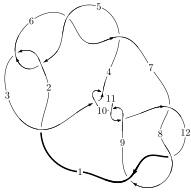
\includegraphics[width=112pt]{../../../GIT/diagram.site/Diagrams/png/1225_12a_0424.png}\\
\ \ \ A knot diagram\footnotemark}&
\allowdisplaybreaks
\textbf{Linearized knot diagam} \\
\cline{2-2}
 &
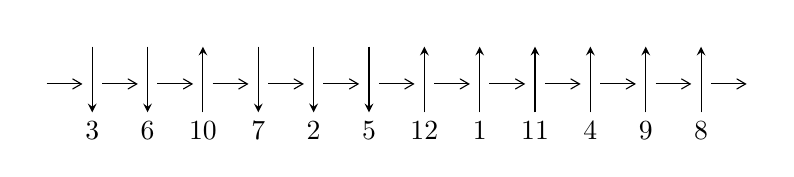
\begin{tikzpicture}[x=20pt, y=17pt]
	% nodes
	\node (C0) at (0, 0) {};
	\node (C1) at (1, 0) {};
	\node (C1U) at (1, +1) {};
	\node (C1D) at (1, -1) {3};

	\node (C2) at (2, 0) {};
	\node (C2U) at (2, +1) {};
	\node (C2D) at (2, -1) {6};

	\node (C3) at (3, 0) {};
	\node (C3U) at (3, +1) {};
	\node (C3D) at (3, -1) {10};

	\node (C4) at (4, 0) {};
	\node (C4U) at (4, +1) {};
	\node (C4D) at (4, -1) {7};

	\node (C5) at (5, 0) {};
	\node (C5U) at (5, +1) {};
	\node (C5D) at (5, -1) {2};

	\node (C6) at (6, 0) {};
	\node (C6U) at (6, +1) {};
	\node (C6D) at (6, -1) {5};

	\node (C7) at (7, 0) {};
	\node (C7U) at (7, +1) {};
	\node (C7D) at (7, -1) {12};

	\node (C8) at (8, 0) {};
	\node (C8U) at (8, +1) {};
	\node (C8D) at (8, -1) {1};

	\node (C9) at (9, 0) {};
	\node (C9U) at (9, +1) {};
	\node (C9D) at (9, -1) {11};

	\node (C10) at (10, 0) {};
	\node (C10U) at (10, +1) {};
	\node (C10D) at (10, -1) {4};

	\node (C11) at (11, 0) {};
	\node (C11U) at (11, +1) {};
	\node (C11D) at (11, -1) {9};

	\node (C12) at (12, 0) {};
	\node (C12U) at (12, +1) {};
	\node (C12D) at (12, -1) {8};
	\node (C13) at (13, 0) {};

	% arrows
	\draw[->,>={angle 60}]
	(C0) edge (C1) (C1) edge (C2) (C2) edge (C3) (C3) edge (C4) (C4) edge (C5) (C5) edge (C6) (C6) edge (C7) (C7) edge (C8) (C8) edge (C9) (C9) edge (C10) (C10) edge (C11) (C11) edge (C12) (C12) edge (C13) ;	\draw[->,>=stealth]
	(C1U) edge (C1D) (C2U) edge (C2D) (C3D) edge (C3U) (C4U) edge (C4D) (C5U) edge (C5D) (C6U) edge (C6D) (C7D) edge (C7U) (C8D) edge (C8U) (C9D) edge (C9U) (C10D) edge (C10U) (C11D) edge (C11U) (C12D) edge (C12U) ;
	\end{tikzpicture} \\
\hhline{~~} \\& 
\textbf{Solving Sequence} \\ \cline{2-2} 
 &
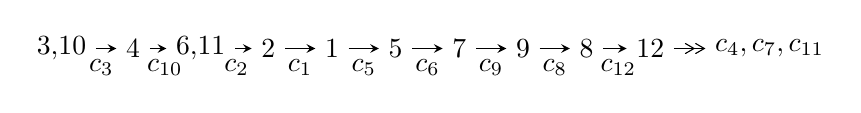
\begin{tikzpicture}[x=23pt, y=7pt]
	% node
	\node (A0) at (-1/8, 0) {3,10};
	\node (A1) at (1, 0) {4};
	\node (A2) at (33/16, 0) {6,11};
	\node (A3) at (25/8, 0) {2};
	\node (A4) at (33/8, 0) {1};
	\node (A5) at (41/8, 0) {5};
	\node (A6) at (49/8, 0) {7};
	\node (A7) at (57/8, 0) {9};
	\node (A8) at (65/8, 0) {8};
	\node (A9) at (73/8, 0) {12};
	\node (C1) at (1/2, -1) {$c_{3}$};
	\node (C2) at (3/2, -1) {$c_{10}$};
	\node (C3) at (21/8, -1) {$c_{2}$};
	\node (C4) at (29/8, -1) {$c_{1}$};
	\node (C5) at (37/8, -1) {$c_{5}$};
	\node (C6) at (45/8, -1) {$c_{6}$};
	\node (C7) at (53/8, -1) {$c_{9}$};
	\node (C8) at (61/8, -1) {$c_{8}$};
	\node (C9) at (69/8, -1) {$c_{12}$};
	\node (A10) at (11, 0) {$c_{4},c_{7},c_{11}$};

	% edge
	\draw[->,>=stealth]	
	(A0) edge (A1) (A1) edge (A2) (A2) edge (A3) (A3) edge (A4) (A4) edge (A5) (A5) edge (A6) (A6) edge (A7) (A7) edge (A8) (A8) edge (A9) ;
	\draw[->>,>={angle 60}]	
	(A9) edge (A10);
\end{tikzpicture} \\ 

\end{tabular} \\

\footnotetext{
The image of knot diagram is generated by the software ``\textbf{Draw programme}" developed by Andrew Bartholomew(\url{http://www.layer8.co.uk/maths/draw/index.htm\#Running-draw}), where we modified some parts for our purpose(\url{https://github.com/CATsTAILs/LinksPainter}).
}\phantom \\ \newline 
\centering \textbf{Ideals for irreducible components\footnotemark of $X_{\text{par}}$} 
 
\begin{align*}
I^u_{1}&=\langle 
-6.05060\times10^{58} u^{67}-1.04724\times10^{59} u^{66}+\cdots+1.01515\times10^{59} b+8.01162\times10^{59},\\
\phantom{I^u_{1}}&\phantom{= \langle  }7.86149\times10^{58} u^{67}+1.36435\times10^{59} u^{66}+\cdots+3.38385\times10^{58} a-9.50671\times10^{59},\;u^{68}+u^{67}+\cdots-4 u+8\rangle \\
\\
I^v_{1}&=\langle 
a,\;b- v+1,\;v^3-2 v^2+v-1\rangle \\
\end{align*}
\raggedright * 2 irreducible components of $\dim_{\mathbb{C}}=0$, with total 71 representations.\\
\footnotetext{All coefficients of polynomials are rational numbers. But the coefficients are sometimes approximated in decimal forms when there is not enough margin.}
\newpage
\renewcommand{\arraystretch}{1}
\centering \section*{I. $I^u_{1}= \langle -6.05\times10^{58} u^{67}-1.05\times10^{59} u^{66}+\cdots+1.02\times10^{59} b+8.01\times10^{59},\;7.86\times10^{58} u^{67}+1.36\times10^{59} u^{66}+\cdots+3.38\times10^{58} a-9.51\times10^{59},\;u^{68}+u^{67}+\cdots-4 u+8 \rangle$}
\flushleft \textbf{(i) Arc colorings}\\
\begin{tabular}{m{7pt} m{180pt} m{7pt} m{180pt} }
\flushright $a_{3}=$&$\begin{pmatrix}1\\0\end{pmatrix}$ \\
\flushright $a_{10}=$&$\begin{pmatrix}0\\u\end{pmatrix}$ \\
\flushright $a_{4}=$&$\begin{pmatrix}1\\- u^2\end{pmatrix}$ \\
\flushright $a_{6}=$&$\begin{pmatrix}-2.32324 u^{67}-4.03195 u^{66}+\cdots+33.5515 u+28.0944\\0.596027 u^{67}+1.03160 u^{66}+\cdots-6.46797 u-7.89203\end{pmatrix}$ \\
\flushright $a_{11}=$&$\begin{pmatrix}u\\- u^3+u\end{pmatrix}$ \\
\flushright $a_{2}=$&$\begin{pmatrix}-1.77029 u^{67}-2.91509 u^{66}+\cdots+24.3748 u+22.7432\\0.564882 u^{67}+0.682242 u^{66}+\cdots-5.65045 u-4.24863\end{pmatrix}$ \\
\flushright $a_{1}=$&$\begin{pmatrix}-1.20541 u^{67}-2.23285 u^{66}+\cdots+18.7243 u+18.4946\\0.564882 u^{67}+0.682242 u^{66}+\cdots-5.65045 u-4.24863\end{pmatrix}$ \\
\flushright $a_{5}=$&$\begin{pmatrix}-0.694072 u^{67}-1.44115 u^{66}+\cdots+11.5944 u+11.4434\\0.204815 u^{67}+0.394112 u^{66}+\cdots-0.0438270 u-5.62061\end{pmatrix}$ \\
\flushright $a_{7}=$&$\begin{pmatrix}-1.77029 u^{67}-2.91509 u^{66}+\cdots+24.3748 u+22.7432\\0.269738 u^{67}+0.621521 u^{66}+\cdots-3.93271 u-4.90972\end{pmatrix}$ \\
\flushright $a_{9}=$&$\begin{pmatrix}- u^3\\u^5- u^3+u\end{pmatrix}$ \\
\flushright $a_{8}=$&$\begin{pmatrix}1.22840 u^{67}+2.01698 u^{66}+\cdots-18.5328 u-16.9508\\-0.265656 u^{67}-0.556698 u^{66}+\cdots+4.05685 u+6.12494\end{pmatrix}$ \\
\flushright $a_{12}=$&$\begin{pmatrix}u^5+u\\- u^7+u^5-2 u^3+u\end{pmatrix}$\\&\end{tabular}
\flushleft \textbf{(ii) Obstruction class $= -1$}\\~\\
\flushleft \textbf{(iii) Cusp Shapes $= -1.40934 u^{67}-1.84025 u^{66}+\cdots+36.8272 u+15.8368$}\\~\\
\newpage\renewcommand{\arraystretch}{1}
\flushleft \textbf{(iv) u-Polynomials at the component}\newline \\
\begin{tabular}{m{50pt}|m{274pt}}
Crossings & \hspace{64pt}u-Polynomials at each crossing \\
\hline $$\begin{aligned}c_{1},c_{4},c_{6}\end{aligned}$$&$\begin{aligned}
&u^{68}+18 u^{67}+\cdots+11 u+1
\end{aligned}$\\
\hline $$\begin{aligned}c_{2},c_{5}\end{aligned}$$&$\begin{aligned}
&u^{68}+2 u^{67}+\cdots+3 u-1
\end{aligned}$\\
\hline $$\begin{aligned}c_{3},c_{10}\end{aligned}$$&$\begin{aligned}
&u^{68}+u^{67}+\cdots-4 u+8
\end{aligned}$\\
\hline $$\begin{aligned}c_{7},c_{8},c_{12}\end{aligned}$$&$\begin{aligned}
&u^{68}+4 u^{67}+\cdots-8 u^2-1
\end{aligned}$\\
\hline $$\begin{aligned}c_{9},c_{11}\end{aligned}$$&$\begin{aligned}
&u^{68}-21 u^{67}+\cdots-720 u+64
\end{aligned}$\\
\hline
\end{tabular}\\~\\
\newpage\renewcommand{\arraystretch}{1}
\flushleft \textbf{(v) Riley Polynomials at the component}\newline \\
\begin{tabular}{m{50pt}|m{274pt}}
Crossings & \hspace{64pt}Riley Polynomials at each crossing \\
\hline $$\begin{aligned}c_{1},c_{4},c_{6}\end{aligned}$$&$\begin{aligned}
&y^{68}+66 y^{67}+\cdots-19 y+1
\end{aligned}$\\
\hline $$\begin{aligned}c_{2},c_{5}\end{aligned}$$&$\begin{aligned}
&y^{68}-18 y^{67}+\cdots-11 y+1
\end{aligned}$\\
\hline $$\begin{aligned}c_{3},c_{10}\end{aligned}$$&$\begin{aligned}
&y^{68}-21 y^{67}+\cdots-720 y+64
\end{aligned}$\\
\hline $$\begin{aligned}c_{7},c_{8},c_{12}\end{aligned}$$&$\begin{aligned}
&y^{68}-56 y^{67}+\cdots+16 y+1
\end{aligned}$\\
\hline $$\begin{aligned}c_{9},c_{11}\end{aligned}$$&$\begin{aligned}
&y^{68}+47 y^{67}+\cdots-19712 y+4096
\end{aligned}$\\
\hline
\end{tabular}\\~\\
\newpage\flushleft \textbf{(vi) Complex Volumes and Cusp Shapes}
$$\begin{array}{c|c|c}  
\text{Solutions to }I^u_{1}& \I (\text{vol} + \sqrt{-1}CS) & \text{Cusp shape}\\
 \hline 
\begin{aligned}
u &= \phantom{-}0.993071 + 0.113125 I \\
a &= -1.89033 - 2.06207 I \\
b &= \phantom{-}0.881273 + 0.827269 I\end{aligned}
 & \phantom{-}6.85914 - 0.90233 I & \phantom{-}8.48968 - 1.09090 I \\ \hline\begin{aligned}
u &= \phantom{-}0.993071 - 0.113125 I \\
a &= -1.89033 + 2.06207 I \\
b &= \phantom{-}0.881273 - 0.827269 I\end{aligned}
 & \phantom{-}6.85914 + 0.90233 I & \phantom{-}8.48968 + 1.09090 I \\ \hline\begin{aligned}
u &= \phantom{-}0.659498 + 0.764722 I \\
a &= \phantom{-}0.550961 + 0.309922 I \\
b &= \phantom{-}0.040503 - 0.569798 I\end{aligned}
 & \phantom{-}0.588563 - 1.246350 I & \phantom{-}5.81021 + 0.45012 I \\ \hline\begin{aligned}
u &= \phantom{-}0.659498 - 0.764722 I \\
a &= \phantom{-}0.550961 - 0.309922 I \\
b &= \phantom{-}0.040503 + 0.569798 I\end{aligned}
 & \phantom{-}0.588563 + 1.246350 I & \phantom{-}5.81021 - 0.45012 I \\ \hline\begin{aligned}
u &= -1.000140 + 0.155243 I \\
a &= -0.98075 - 2.90583 I \\
b &= \phantom{-}0.913795 + 0.817365 I\end{aligned}
 & \phantom{-}6.75864 - 5.23492 I & \phantom{-}7.99359 + 6.56298 I \\ \hline\begin{aligned}
u &= -1.000140 - 0.155243 I \\
a &= -0.98075 + 2.90583 I \\
b &= \phantom{-}0.913795 - 0.817365 I\end{aligned}
 & \phantom{-}6.75864 + 5.23492 I & \phantom{-}7.99359 - 6.56298 I \\ \hline\begin{aligned}
u &= \phantom{-}0.021687 + 1.023690 I \\
a &= -0.218747 + 0.841325 I \\
b &= -0.898997 - 0.825730 I\end{aligned}
 & \phantom{-}8.72956 - 3.07936 I & \phantom{-}8.43070 + 2.69230 I \\ \hline\begin{aligned}
u &= \phantom{-}0.021687 - 1.023690 I \\
a &= -0.218747 - 0.841325 I \\
b &= -0.898997 + 0.825730 I\end{aligned}
 & \phantom{-}8.72956 + 3.07936 I & \phantom{-}8.43070 - 2.69230 I \\ \hline\begin{aligned}
u &= \phantom{-}0.991893 + 0.263165 I \\
a &= -0.412778 - 1.347760 I \\
b &= -0.884341 + 0.498364 I\end{aligned}
 & \phantom{-}5.18458 + 4.97460 I & \phantom{-}7.77509 - 7.49917 I \\ \hline\begin{aligned}
u &= \phantom{-}0.991893 - 0.263165 I \\
a &= -0.412778 + 1.347760 I \\
b &= -0.884341 - 0.498364 I\end{aligned}
 & \phantom{-}5.18458 - 4.97460 I & \phantom{-}7.77509 + 7.49917 I\\
 \hline 
 \end{array}$$\newpage$$\begin{array}{c|c|c}  
\text{Solutions to }I^u_{1}& \I (\text{vol} + \sqrt{-1}CS) & \text{Cusp shape}\\
 \hline 
\begin{aligned}
u &= -0.829279 + 0.618745 I \\
a &= -0.332097 - 0.896610 I \\
b &= -0.970966 + 0.736214 I\end{aligned}
 & \phantom{-}3.84635 + 0.92115 I & \phantom{-}5.28354 + 1.08542 I \\ \hline\begin{aligned}
u &= -0.829279 - 0.618745 I \\
a &= -0.332097 + 0.896610 I \\
b &= -0.970966 - 0.736214 I\end{aligned}
 & \phantom{-}3.84635 - 0.92115 I & \phantom{-}5.28354 - 1.08542 I \\ \hline\begin{aligned}
u &= -0.697002 + 0.783946 I \\
a &= -0.105875 + 0.873399 I \\
b &= -0.785825 - 0.814885 I\end{aligned}
 & \phantom{-}0.83003 - 1.22443 I & \phantom{-}2.00000 + 2.28588 I \\ \hline\begin{aligned}
u &= -0.697002 - 0.783946 I \\
a &= -0.105875 - 0.873399 I \\
b &= -0.785825 + 0.814885 I\end{aligned}
 & \phantom{-}0.83003 + 1.22443 I & \phantom{-}2.00000 - 2.28588 I \\ \hline\begin{aligned}
u &= \phantom{-}0.884256 + 0.567359 I \\
a &= -0.044342 - 0.919731 I \\
b &= -0.732492 + 0.772305 I\end{aligned}
 & \phantom{-}4.53565 + 4.78229 I & \phantom{-}7.19204 - 6.23856 I \\ \hline\begin{aligned}
u &= \phantom{-}0.884256 - 0.567359 I \\
a &= -0.044342 + 0.919731 I \\
b &= -0.732492 - 0.772305 I\end{aligned}
 & \phantom{-}4.53565 - 4.78229 I & \phantom{-}7.19204 + 6.23856 I \\ \hline\begin{aligned}
u &= -1.061960 + 0.111325 I \\
a &= \phantom{-}0.459698 - 0.837106 I \\
b &= -0.392765 + 0.607634 I\end{aligned}
 & \phantom{-}6.64379 - 0.94912 I & \phantom{-}11.95029 + 0. I\phantom{ +0.000000I} \\ \hline\begin{aligned}
u &= -1.061960 - 0.111325 I \\
a &= \phantom{-}0.459698 + 0.837106 I \\
b &= -0.392765 - 0.607634 I\end{aligned}
 & \phantom{-}6.64379 + 0.94912 I & \phantom{-}11.95029 + 0. I\phantom{ +0.000000I} \\ \hline\begin{aligned}
u &= \phantom{-}0.890731 + 0.590142 I \\
a &= -1.76219 - 0.11747 I \\
b &= \phantom{-}0.809278 + 0.829802 I\end{aligned}
 & \phantom{-}4.59428 - 0.22084 I & \phantom{-}6.48510 + 0. I\phantom{ +0.000000I} \\ \hline\begin{aligned}
u &= \phantom{-}0.890731 - 0.590142 I \\
a &= -1.76219 + 0.11747 I \\
b &= \phantom{-}0.809278 - 0.829802 I\end{aligned}
 & \phantom{-}4.59428 + 0.22084 I & \phantom{-}6.48510 + 0. I\phantom{ +0.000000I}\\
 \hline 
 \end{array}$$\newpage$$\begin{array}{c|c|c}  
\text{Solutions to }I^u_{1}& \I (\text{vol} + \sqrt{-1}CS) & \text{Cusp shape}\\
 \hline 
\begin{aligned}
u &= \phantom{-}0.716202 + 0.821100 I \\
a &= -0.311479 + 0.865388 I \\
b &= -0.969652 - 0.768571 I\end{aligned}
 & \phantom{-}0.27108 - 4.71837 I & \phantom{-0.000000 } 0 \\ \hline\begin{aligned}
u &= \phantom{-}0.716202 - 0.821100 I \\
a &= -0.311479 - 0.865388 I \\
b &= -0.969652 + 0.768571 I\end{aligned}
 & \phantom{-}0.27108 + 4.71837 I & \phantom{-0.000000 } 0 \\ \hline\begin{aligned}
u &= -0.800894 + 0.745034 I \\
a &= -1.40099 + 1.63231 I \\
b &= -0.971234 - 0.263287 I\end{aligned}
 & -2.36206 - 1.49059 I & \phantom{-0.000000 } 0 \\ \hline\begin{aligned}
u &= -0.800894 - 0.745034 I \\
a &= -1.40099 - 1.63231 I \\
b &= -0.971234 + 0.263287 I\end{aligned}
 & -2.36206 + 1.49059 I & \phantom{-0.000000 } 0 \\ \hline\begin{aligned}
u &= -0.909702 + 0.630284 I \\
a &= \phantom{-}0.94341 - 2.77762 I \\
b &= \phantom{-}0.964261 + 0.783946 I\end{aligned}
 & \phantom{-}4.11637 - 5.81729 I & \phantom{-0.000000 } 0 \\ \hline\begin{aligned}
u &= -0.909702 - 0.630284 I \\
a &= \phantom{-}0.94341 + 2.77762 I \\
b &= \phantom{-}0.964261 - 0.783946 I\end{aligned}
 & \phantom{-}4.11637 + 5.81729 I & \phantom{-0.000000 } 0 \\ \hline\begin{aligned}
u &= \phantom{-}0.876321\phantom{ +0.000000I} \\
a &= \phantom{-}0.998697\phantom{ +0.000000I} \\
b &= \phantom{-}0.963850\phantom{ +0.000000I}\end{aligned}
 & \phantom{-}2.31122\phantom{ +0.000000I} & \phantom{-}4.45630\phantom{ +0.000000I} \\ \hline\begin{aligned}
u &= -0.867744 + 0.719052 I \\
a &= \phantom{-}0.502678 - 0.415224 I \\
b &= -0.051505 + 0.630284 I\end{aligned}
 & -2.78825 - 2.74528 I & \phantom{-0.000000 } 0 \\ \hline\begin{aligned}
u &= -0.867744 - 0.719052 I \\
a &= \phantom{-}0.502678 + 0.415224 I \\
b &= -0.051505 - 0.630284 I\end{aligned}
 & -2.78825 + 2.74528 I & \phantom{-0.000000 } 0 \\ \hline\begin{aligned}
u &= -0.723892 + 0.871174 I \\
a &= \phantom{-}1.099390 - 0.016027 I \\
b &= \phantom{-}0.977262 - 0.289069 I\end{aligned}
 & -2.20577 + 4.23347 I & \phantom{-0.000000 } 0\\
 \hline 
 \end{array}$$\newpage$$\begin{array}{c|c|c}  
\text{Solutions to }I^u_{1}& \I (\text{vol} + \sqrt{-1}CS) & \text{Cusp shape}\\
 \hline 
\begin{aligned}
u &= -0.723892 - 0.871174 I \\
a &= \phantom{-}1.099390 + 0.016027 I \\
b &= \phantom{-}0.977262 + 0.289069 I\end{aligned}
 & -2.20577 - 4.23347 I & \phantom{-0.000000 } 0 \\ \hline\begin{aligned}
u &= \phantom{-}0.829532 + 0.792287 I \\
a &= \phantom{-}1.069520 + 0.001488 I \\
b &= \phantom{-}0.995888 + 0.247406 I\end{aligned}
 & -6.00877 - 0.07335 I & \phantom{-0.000000 } 0 \\ \hline\begin{aligned}
u &= \phantom{-}0.829532 - 0.792287 I \\
a &= \phantom{-}1.069520 - 0.001488 I \\
b &= \phantom{-}0.995888 - 0.247406 I\end{aligned}
 & -6.00877 + 0.07335 I & \phantom{-0.000000 } 0 \\ \hline\begin{aligned}
u &= \phantom{-}0.637253 + 0.973593 I \\
a &= -0.123805 - 0.840626 I \\
b &= -0.805330 + 0.845791 I\end{aligned}
 & \phantom{-}5.07615 - 2.51950 I & \phantom{-0.000000 } 0 \\ \hline\begin{aligned}
u &= \phantom{-}0.637253 - 0.973593 I \\
a &= -0.123805 + 0.840626 I \\
b &= -0.805330 - 0.845791 I\end{aligned}
 & \phantom{-}5.07615 + 2.51950 I & \phantom{-0.000000 } 0 \\ \hline\begin{aligned}
u &= -0.781819 + 0.294985 I \\
a &= -0.05603 + 1.97815 I \\
b &= -0.755261 - 0.362856 I\end{aligned}
 & \phantom{-}0.13820 - 2.92436 I & \phantom{-}2.59443 + 9.53509 I \\ \hline\begin{aligned}
u &= -0.781819 - 0.294985 I \\
a &= -0.05603 - 1.97815 I \\
b &= -0.755261 + 0.362856 I\end{aligned}
 & \phantom{-}0.13820 + 2.92436 I & \phantom{-}2.59443 - 9.53509 I \\ \hline\begin{aligned}
u &= -0.933508 + 0.715246 I \\
a &= \phantom{-}1.048350 + 0.008631 I \\
b &= \phantom{-}1.016160 - 0.211403 I\end{aligned}
 & -1.94942 - 4.06921 I & \phantom{-0.000000 } 0 \\ \hline\begin{aligned}
u &= -0.933508 - 0.715246 I \\
a &= \phantom{-}1.048350 - 0.008631 I \\
b &= \phantom{-}1.016160 + 0.211403 I\end{aligned}
 & -1.94942 + 4.06921 I & \phantom{-0.000000 } 0 \\ \hline\begin{aligned}
u &= -0.667756 + 0.982329 I \\
a &= -0.302229 - 0.843220 I \\
b &= -0.972548 + 0.790652 I\end{aligned}
 & \phantom{-}4.55831 + 8.62464 I & \phantom{-0.000000 } 0\\
 \hline 
 \end{array}$$\newpage$$\begin{array}{c|c|c}  
\text{Solutions to }I^u_{1}& \I (\text{vol} + \sqrt{-1}CS) & \text{Cusp shape}\\
 \hline 
\begin{aligned}
u &= -0.667756 - 0.982329 I \\
a &= -0.302229 + 0.843220 I \\
b &= -0.972548 - 0.790652 I\end{aligned}
 & \phantom{-}4.55831 - 8.62464 I & \phantom{-0.000000 } 0 \\ \hline\begin{aligned}
u &= \phantom{-}0.923270 + 0.765436 I \\
a &= -1.25292 - 1.44461 I \\
b &= -0.999457 + 0.296326 I\end{aligned}
 & -5.71945 + 5.92897 I & \phantom{-0.000000 } 0 \\ \hline\begin{aligned}
u &= \phantom{-}0.923270 - 0.765436 I \\
a &= -1.25292 + 1.44461 I \\
b &= -0.999457 - 0.296326 I\end{aligned}
 & -5.71945 - 5.92897 I & \phantom{-0.000000 } 0 \\ \hline\begin{aligned}
u &= -0.996451 + 0.711234 I \\
a &= -1.309380 + 0.201391 I \\
b &= \phantom{-}0.794344 - 0.853811 I\end{aligned}
 & \phantom{-}1.73332 - 4.42504 I & \phantom{-0.000000 } 0 \\ \hline\begin{aligned}
u &= -0.996451 - 0.711234 I \\
a &= -1.309380 - 0.201391 I \\
b &= \phantom{-}0.794344 + 0.853811 I\end{aligned}
 & \phantom{-}1.73332 + 4.42504 I & \phantom{-0.000000 } 0 \\ \hline\begin{aligned}
u &= \phantom{-}0.170683 + 0.754290 I \\
a &= \phantom{-}0.848846 + 0.211083 I \\
b &= \phantom{-}0.635194 + 0.359962 I\end{aligned}
 & \phantom{-}2.32891 - 1.45239 I & \phantom{-}4.90559 + 4.31092 I \\ \hline\begin{aligned}
u &= \phantom{-}0.170683 - 0.754290 I \\
a &= \phantom{-}0.848846 - 0.211083 I \\
b &= \phantom{-}0.635194 - 0.359962 I\end{aligned}
 & \phantom{-}2.32891 + 1.45239 I & \phantom{-}4.90559 - 4.31092 I \\ \hline\begin{aligned}
u &= \phantom{-}1.008450 + 0.698435 I \\
a &= \phantom{-}0.456475 + 0.467018 I \\
b &= -0.098986 - 0.677355 I\end{aligned}
 & \phantom{-}1.62108 + 6.80691 I & \phantom{-0.000000 } 0 \\ \hline\begin{aligned}
u &= \phantom{-}1.008450 - 0.698435 I \\
a &= \phantom{-}0.456475 - 0.467018 I \\
b &= -0.098986 + 0.677355 I\end{aligned}
 & \phantom{-}1.62108 - 6.80691 I & \phantom{-0.000000 } 0 \\ \hline\begin{aligned}
u &= \phantom{-}1.003540 + 0.733346 I \\
a &= \phantom{-}0.89900 + 2.36045 I \\
b &= \phantom{-}0.981570 - 0.789856 I\end{aligned}
 & \phantom{-}1.15325 + 10.54940 I & \phantom{-0.000000 } 0\\
 \hline 
 \end{array}$$\newpage$$\begin{array}{c|c|c}  
\text{Solutions to }I^u_{1}& \I (\text{vol} + \sqrt{-1}CS) & \text{Cusp shape}\\
 \hline 
\begin{aligned}
u &= \phantom{-}1.003540 - 0.733346 I \\
a &= \phantom{-}0.89900 - 2.36045 I \\
b &= \phantom{-}0.981570 + 0.789856 I\end{aligned}
 & \phantom{-}1.15325 - 10.54940 I & \phantom{-0.000000 } 0 \\ \hline\begin{aligned}
u &= -1.234530 + 0.258857 I \\
a &= -1.25723 + 1.36690 I \\
b &= \phantom{-}0.873045 - 0.864648 I\end{aligned}
 & \phantom{-}13.36960 - 1.32073 I & \phantom{-0.000000 } 0 \\ \hline\begin{aligned}
u &= -1.234530 - 0.258857 I \\
a &= -1.25723 - 1.36690 I \\
b &= \phantom{-}0.873045 + 0.864648 I\end{aligned}
 & \phantom{-}13.36960 + 1.32073 I & \phantom{-0.000000 } 0 \\ \hline\begin{aligned}
u &= \phantom{-}1.231130 + 0.291396 I \\
a &= -0.32877 + 2.27833 I \\
b &= \phantom{-}0.940263 - 0.838288 I\end{aligned}
 & \phantom{-}13.1585 + 7.6380 I & \phantom{-0.000000 } 0 \\ \hline\begin{aligned}
u &= \phantom{-}1.231130 - 0.291396 I \\
a &= -0.32877 - 2.27833 I \\
b &= \phantom{-}0.940263 + 0.838288 I\end{aligned}
 & \phantom{-}13.1585 - 7.6380 I & \phantom{-0.000000 } 0 \\ \hline\begin{aligned}
u &= -1.017380 + 0.758083 I \\
a &= -1.15099 + 1.34572 I \\
b &= -1.016370 - 0.322893 I\end{aligned}
 & -1.29085 - 10.28430 I & \phantom{-0.000000 } 0 \\ \hline\begin{aligned}
u &= -1.017380 - 0.758083 I \\
a &= -1.15099 - 1.34572 I \\
b &= -1.016370 + 0.322893 I\end{aligned}
 & -1.29085 + 10.28430 I & \phantom{-0.000000 } 0 \\ \hline\begin{aligned}
u &= \phantom{-}0.676957 + 0.032911 I \\
a &= \phantom{-}1.18518 + 1.04468 I \\
b &= -0.420279 - 0.292993 I\end{aligned}
 & \phantom{-}1.049650 + 0.101234 I & \phantom{-}9.47396 - 0.04712 I \\ \hline\begin{aligned}
u &= \phantom{-}0.676957 - 0.032911 I \\
a &= \phantom{-}1.18518 - 1.04468 I \\
b &= -0.420279 + 0.292993 I\end{aligned}
 & \phantom{-}1.049650 - 0.101234 I & \phantom{-}9.47396 + 0.04712 I \\ \hline\begin{aligned}
u &= \phantom{-}1.094230 + 0.755851 I \\
a &= -1.129750 - 0.325888 I \\
b &= \phantom{-}0.793548 + 0.872752 I\end{aligned}
 & \phantom{-}6.52598 + 8.82716 I & \phantom{-0.000000 } 0\\
 \hline 
 \end{array}$$\newpage$$\begin{array}{c|c|c}  
\text{Solutions to }I^u_{1}& \I (\text{vol} + \sqrt{-1}CS) & \text{Cusp shape}\\
 \hline 
\begin{aligned}
u &= \phantom{-}1.094230 - 0.755851 I \\
a &= -1.129750 + 0.325888 I \\
b &= \phantom{-}0.793548 - 0.872752 I\end{aligned}
 & \phantom{-}6.52598 - 8.82716 I & \phantom{-0.000000 } 0 \\ \hline\begin{aligned}
u &= -1.091090 + 0.774273 I \\
a &= \phantom{-}0.79093 - 2.16616 I \\
b &= \phantom{-}0.990918 + 0.798516 I\end{aligned}
 & \phantom{-}5.9100 - 15.0350 I & \phantom{-0.000000 } 0 \\ \hline\begin{aligned}
u &= -1.091090 - 0.774273 I \\
a &= \phantom{-}0.79093 + 2.16616 I \\
b &= \phantom{-}0.990918 - 0.798516 I\end{aligned}
 & \phantom{-}5.9100 + 15.0350 I & \phantom{-0.000000 } 0 \\ \hline\begin{aligned}
u &= -0.022492 + 0.551897 I \\
a &= -0.220910 - 0.899639 I \\
b &= -0.884082 + 0.773478 I\end{aligned}
 & \phantom{-}3.60354 + 2.91698 I & -1.07047 - 2.93516 I \\ \hline\begin{aligned}
u &= -0.022492 - 0.551897 I \\
a &= -0.220910 + 0.899639 I \\
b &= -0.884082 - 0.773478 I\end{aligned}
 & \phantom{-}3.60354 - 2.91698 I & -1.07047 + 2.93516 I \\ \hline\begin{aligned}
u &= \phantom{-}0.528183\phantom{ +0.000000I} \\
a &= \phantom{-}2.56903\phantom{ +0.000000I} \\
b &= -0.477187\phantom{ +0.000000I}\end{aligned}
 & \phantom{-}1.06452\phantom{ +0.000000I} & \phantom{-}11.9270\phantom{ +0.000000I} \\ \hline\begin{aligned}
u &= -0.298991 + 0.383237 I \\
a &= \phantom{-}0.953304 - 0.043713 I \\
b &= \phantom{-}0.759455 - 0.112169 I\end{aligned}
 & -1.254010 + 0.311770 I & -6.76966 - 0.58136 I \\ \hline\begin{aligned}
u &= -0.298991 - 0.383237 I \\
a &= \phantom{-}0.953304 + 0.043713 I \\
b &= \phantom{-}0.759455 + 0.112169 I\end{aligned}
 & -1.254010 - 0.311770 I & -6.76966 + 0.58136 I\\
 \hline 
 \end{array}$$\newpage\newpage\renewcommand{\arraystretch}{1}
\centering \section*{II. $I^v_{1}= \langle a,\;b- v+1,\;v^3-2 v^2+v-1 \rangle$}
\flushleft \textbf{(i) Arc colorings}\\
\begin{tabular}{m{7pt} m{180pt} m{7pt} m{180pt} }
\flushright $a_{3}=$&$\begin{pmatrix}1\\0\end{pmatrix}$ \\
\flushright $a_{10}=$&$\begin{pmatrix}v\\0\end{pmatrix}$ \\
\flushright $a_{4}=$&$\begin{pmatrix}1\\0\end{pmatrix}$ \\
\flushright $a_{6}=$&$\begin{pmatrix}0\\v-1\end{pmatrix}$ \\
\flushright $a_{11}=$&$\begin{pmatrix}v\\0\end{pmatrix}$ \\
\flushright $a_{2}=$&$\begin{pmatrix}1\\- v^2+2 v-1\end{pmatrix}$ \\
\flushright $a_{1}=$&$\begin{pmatrix}- v^2+2 v\\- v^2+2 v-1\end{pmatrix}$ \\
\flushright $a_{5}=$&$\begin{pmatrix}v-1\\v^2- v-1\end{pmatrix}$ \\
\flushright $a_{7}=$&$\begin{pmatrix}v^2-2 v\\v^2-2 v+1\end{pmatrix}$ \\
\flushright $a_{9}=$&$\begin{pmatrix}v\\0\end{pmatrix}$ \\
\flushright $a_{8}=$&$\begin{pmatrix}v^2- v\\v^2-2 v+1\end{pmatrix}$ \\
\flushright $a_{12}=$&$\begin{pmatrix}v\\0\end{pmatrix}$\\&\end{tabular}
\flushleft \textbf{(ii) Obstruction class $= 1$}\\~\\
\flushleft \textbf{(iii) Cusp Shapes $= -2 v^2-3 v+7$}\\~\\
\newpage\renewcommand{\arraystretch}{1}
\flushleft \textbf{(iv) u-Polynomials at the component}\newline \\
\begin{tabular}{m{50pt}|m{274pt}}
Crossings & \hspace{64pt}u-Polynomials at each crossing \\
\hline $$\begin{aligned}c_{1},c_{4}\end{aligned}$$&$\begin{aligned}
&u^3- u^2+2 u-1
\end{aligned}$\\
\hline $$\begin{aligned}c_{2}\end{aligned}$$&$\begin{aligned}
&u^3+u^2-1
\end{aligned}$\\
\hline $$\begin{aligned}c_{3},c_{9},c_{10}\\c_{11}\end{aligned}$$&$\begin{aligned}
&u^3
\end{aligned}$\\
\hline $$\begin{aligned}c_{5}\end{aligned}$$&$\begin{aligned}
&u^3- u^2+1
\end{aligned}$\\
\hline $$\begin{aligned}c_{6}\end{aligned}$$&$\begin{aligned}
&u^3+u^2+2 u+1
\end{aligned}$\\
\hline $$\begin{aligned}c_{7},c_{8}\end{aligned}$$&$\begin{aligned}
&(u+1)^3
\end{aligned}$\\
\hline $$\begin{aligned}c_{12}\end{aligned}$$&$\begin{aligned}
&(u-1)^3
\end{aligned}$\\
\hline
\end{tabular}\\~\\
\newpage\renewcommand{\arraystretch}{1}
\flushleft \textbf{(v) Riley Polynomials at the component}\newline \\
\begin{tabular}{m{50pt}|m{274pt}}
Crossings & \hspace{64pt}Riley Polynomials at each crossing \\
\hline $$\begin{aligned}c_{1},c_{4},c_{6}\end{aligned}$$&$\begin{aligned}
&y^3+3 y^2+2 y-1
\end{aligned}$\\
\hline $$\begin{aligned}c_{2},c_{5}\end{aligned}$$&$\begin{aligned}
&y^3- y^2+2 y-1
\end{aligned}$\\
\hline $$\begin{aligned}c_{3},c_{9},c_{10}\\c_{11}\end{aligned}$$&$\begin{aligned}
&y^3
\end{aligned}$\\
\hline $$\begin{aligned}c_{7},c_{8},c_{12}\end{aligned}$$&$\begin{aligned}
&(y-1)^3
\end{aligned}$\\
\hline
\end{tabular}\\~\\
\newpage\flushleft \textbf{(vi) Complex Volumes and Cusp Shapes}
$$\begin{array}{c|c|c}  
\text{Solutions to }I^v_{1}& \I (\text{vol} + \sqrt{-1}CS) & \text{Cusp shape}\\
 \hline 
\begin{aligned}
v &= \phantom{-}0.122561 + 0.744862 I \\
a &= \phantom{-0.000000 } 0 \\
b &= -0.877439 + 0.744862 I\end{aligned}
 & \phantom{-}4.66906 + 2.82812 I & \phantom{-}7.71191 - 2.59975 I \\ \hline\begin{aligned}
v &= \phantom{-}0.122561 - 0.744862 I \\
a &= \phantom{-0.000000 } 0 \\
b &= -0.877439 - 0.744862 I\end{aligned}
 & \phantom{-}4.66906 - 2.82812 I & \phantom{-}7.71191 + 2.59975 I \\ \hline\begin{aligned}
v &= \phantom{-}1.75488\phantom{ +0.000000I} \\
a &= \phantom{-0.000000 } 0 \\
b &= \phantom{-}0.754878\phantom{ +0.000000I}\end{aligned}
 & \phantom{-}0.531480\phantom{ +0.000000I} & -4.42380\phantom{ +0.000000I}\\
 \hline 
 \end{array}$$\newpage
\newpage\renewcommand{\arraystretch}{1}
\centering \section*{ III. u-Polynomials}
\begin{tabular}{m{50pt}|m{274pt}}
Crossings & \hspace{64pt}u-Polynomials at each crossing \\
\hline $$\begin{aligned}c_{1},c_{4}\end{aligned}$$&$\begin{aligned}
&(u^3- u^2+2 u-1)(u^{68}+18 u^{67}+\cdots+11 u+1)
\end{aligned}$\\
\hline $$\begin{aligned}c_{2}\end{aligned}$$&$\begin{aligned}
&(u^3+u^2-1)(u^{68}+2 u^{67}+\cdots+3 u-1)
\end{aligned}$\\
\hline $$\begin{aligned}c_{3},c_{10}\end{aligned}$$&$\begin{aligned}
&u^3(u^{68}+u^{67}+\cdots-4 u+8)
\end{aligned}$\\
\hline $$\begin{aligned}c_{5}\end{aligned}$$&$\begin{aligned}
&(u^3- u^2+1)(u^{68}+2 u^{67}+\cdots+3 u-1)
\end{aligned}$\\
\hline $$\begin{aligned}c_{6}\end{aligned}$$&$\begin{aligned}
&(u^3+u^2+2 u+1)(u^{68}+18 u^{67}+\cdots+11 u+1)
\end{aligned}$\\
\hline $$\begin{aligned}c_{7},c_{8}\end{aligned}$$&$\begin{aligned}
&((u+1)^3)(u^{68}+4 u^{67}+\cdots-8 u^2-1)
\end{aligned}$\\
\hline $$\begin{aligned}c_{9},c_{11}\end{aligned}$$&$\begin{aligned}
&u^3(u^{68}-21 u^{67}+\cdots-720 u+64)
\end{aligned}$\\
\hline $$\begin{aligned}c_{12}\end{aligned}$$&$\begin{aligned}
&((u-1)^3)(u^{68}+4 u^{67}+\cdots-8 u^2-1)
\end{aligned}$\\
\hline
\end{tabular}\newpage\renewcommand{\arraystretch}{1}
\centering \section*{ IV. Riley Polynomials}
\begin{tabular}{m{50pt}|m{274pt}}
Crossings & \hspace{64pt}Riley Polynomials at each crossing \\
\hline $$\begin{aligned}c_{1},c_{4},c_{6}\end{aligned}$$&$\begin{aligned}
&(y^3+3 y^2+2 y-1)(y^{68}+66 y^{67}+\cdots-19 y+1)
\end{aligned}$\\
\hline $$\begin{aligned}c_{2},c_{5}\end{aligned}$$&$\begin{aligned}
&(y^3- y^2+2 y-1)(y^{68}-18 y^{67}+\cdots-11 y+1)
\end{aligned}$\\
\hline $$\begin{aligned}c_{3},c_{10}\end{aligned}$$&$\begin{aligned}
&y^3(y^{68}-21 y^{67}+\cdots-720 y+64)
\end{aligned}$\\
\hline $$\begin{aligned}c_{7},c_{8},c_{12}\end{aligned}$$&$\begin{aligned}
&((y-1)^3)(y^{68}-56 y^{67}+\cdots+16 y+1)
\end{aligned}$\\
\hline $$\begin{aligned}c_{9},c_{11}\end{aligned}$$&$\begin{aligned}
&y^3(y^{68}+47 y^{67}+\cdots-19712 y+4096)
\end{aligned}$\\
\hline
\end{tabular}
\vskip 2pc
\end{document}